% ============================================================================
% AAAI-27 Chinese mirror draft for internal review.
% The official aaai2027.sty requires pdfLaTeX and cannot typeset CJK.
% This mirror keeps the same two-column content geometry and bibliography
% style, but it is not the submission source.
% Evidence freeze: 2026-07-16.
% Compile: xelatex -> bibtex -> xelatex -> xelatex.
% ============================================================================
\documentclass[UTF8,letterpaper,10pt,twocolumn]{ctexart}
\usepackage[
  letterpaper,
  left=0.75in,
  right=0.75in,
  top=0.75in,
  bottom=0.75in,
  columnsep=0.25in
]{geometry}
\usepackage[hyphens]{url}
\usepackage{graphicx}
\urlstyle{rm}
\def\UrlFont{\rm}
\usepackage{natbib}
\usepackage{caption}
\frenchspacing
\usepackage{booktabs}
\usepackage{amsmath}
\usepackage{array}
\setCJKmainfont[ItalicFont=Microsoft YaHei]{Microsoft YaHei}
\setCJKsansfont{Microsoft YaHei}
\setCJKmonofont{Microsoft YaHei}
\setmainfont{TeX Gyre Termes}
\setsansfont{TeX Gyre Heros}
\setmonofont{TeX Gyre Cursor}
\pagestyle{empty}
\setlength{\parindent}{1em}
\setlength{\parskip}{0pt}
\captionsetup{font=small,labelfont=bf}
\ctexset{
  section = {format=\large\bfseries,beforeskip=8pt,afterskip=4pt},
  subsection = {format=\normalsize\bfseries,beforeskip=6pt,afterskip=3pt}
}

\setcounter{secnumdepth}{2}

\title{当共享经验成为实现吸引子：并行大模型智能体中的锁定、缓解与任务边界}
\author{匿名投稿（中文镜像稿）}
\date{}

\begin{document}
\maketitle

\begin{abstract}
并行大模型智能体通常通过向后续智能体广播先前输出或管理器合成的经验来提升能力。本文审计一种弱于灾难性失败、却更容易被平均分数掩盖的风险：共享经验可能压制独立解，并稳定出共同的实现吸引子。我们构建了一个分层 Mixture-of-Agents 编程系统，每层包含三个私有 MiniSWE 工作区，经验迁移对外部评分盲化，并由隐藏可执行测试进行评估。在冻结的 Kimi-K2.6、12 层、三臂实验中，累积自报告经验没有复现预注册的持续退化曲线；相反，三个智能体从第 3 层起共享同一失败测试签名，从第 5 层起生成完全相同的实现，并一直停留在 33/37。对另外两条独立累积轨迹的回顾性审计分别从第 3 层和第 4 层复现连续的精确快照锁定。一个前瞻冻结的固定三引用对照从第 2--6 层只保留一个主实现，表明累积历史增长并非必要条件。随后，一个只使用本地实现身份的多样性路由器把第 2--6 层多样性 AUC 从 5 提高到 6，并将锁定从第 2 层推迟到第 3 层，全部输出仍为 34/37，但没有阻止锁定。在前瞻冻结、同提供商的 \texttt{log\_query} 边界中，三种策略到第 3 层都保留三个实现，而迁移把平均全测试通过数从 108.4/134 提高到 127.2/134 和 130.1/134。因此，共享经验产生的是有条件的质量--多样性权衡，而不是普适的多智能体“死亡螺旋”。此外，本地“完成声明加冒烟命令”门控拒绝了两个零命令假完成输出，但冻结阈值也误拒了五个强解。
\end{abstract}

\section{引言}

当局部合理的轨迹跟随规则在群体层面形成自我强化时，行军蚁可能进入环形死亡行军~\citep{schneirla1944circularmill}。这一隐喻很容易被套用到多智能体大模型系统：每条被导入的经验都可能看似合理，每个接收者也可能宣称任务已经成功，但反复共享仍可能消除并行智能体原本有价值的独立性。不过，隐喻不是证据。本文提出一个更窄、可执行的问题：\emph{当多个并行编程智能体持续吸收共享经验时，实际会发生什么？}

分层 Mixture-of-Agents（MoA）让多个智能体解决同一任务，并将前层输出提供给后层~\citep{wang2024moa}。经验驱动智能体则从轨迹中提炼可复用的文本指导~\citep{zhao2024expel,shinn2023reflexion}；多智能体软件开发系统进一步共享消息、角色或跨任务经验~\citep{qian2024chatdev,qian2024colearning,li2025mael_full}。这些机制可以提升正确率与效率，也会使接收者相关化：一旦某个共享制品获得特权地位，后续所谓“独立”的智能体可能继承相同的假设、测试方式与遗漏。

近期工作已在多智能体讨论中观察到语义锚定与多样性塌缩~\citep{guo2026diversitycollapse,zhang2026semanticcollapse}。本文关注与之互补的\emph{经验介导锁定}：每个智能体在私有代码仓库中工作，外部测试精确测量行为，目录快照哈希则用于审计实现身份。由此可以区分三个经常被混为一谈的结果：（i）性能坍塌；（ii）实现锁定；（iii）即使代码不同，行为仍然锁定。

我们最初试图寻找一条持续退化曲线：随着经验不断被接纳，正确但愈发复杂的指导可能诱发假完成，并通过共享继续扩散。最强的冻结复现否定了这一叙事。更可复现的发现更细微：累积经验快速同质化行为，有时甚至使代码完全相同；灾难输出则仍然随机、依赖模型并可在下一层恢复。本地接纳规则能够拦截观察到的零命令假完成，但同一阈值也会丢弃强解。两条独立轨迹审计复现了精确实现锁定，固定三引用对照则表明这一现象无需持续增长的历史。递归合成在一个任务上锁定到劣质固定点，却在另一个任务上带来改善。本地多样性路由器在 \texttt{cfgpipe} 上只能推迟一层锁定；同提供商的 \texttt{log\_query} 探针则在迁移提高质量时仍保持最大的实现多样性。

本文贡献如下：
\begin{itemize}
    \item 构建一个带私有工作区、层间屏障、盲化经验迁移、隐藏外部评估和精确经验制品规范的可审计分层 MoA 编程平台；
    \item 给出预注册的负结果：跨三个模型族，深度与上下文增长不能稳定产生持续退化曲线；
    \item 给出可重复的轨迹与源码对齐证据，并以前瞻固定引用对照表明：在所测设置中，累积历史增长不是精确实现锁定的必要条件；
    \item 前瞻评估一个本地多样性路由器，发现它只能将锁定推迟一层；同时给出同提供商第二任务边界，其中迁移提高质量但不降低实现多样性；
    \item 通过轨迹级接纳审计，量化拦截假完成与保留高质量经验之间的权衡。
\end{itemize}

\section{相关工作}

\paragraph{经验型智能体与共享记忆。}
ExpeL 从智能体轨迹中提炼可复用洞见~\citep{zhao2024expel}；Reflexion 保存语言反馈以修正后续尝试~\citep{shinn2023reflexion}；Generative Agents 与 MemoryBank 管理长期检索和显著性~\citep{park2023generative,zhong2024memorybank}。经验协同学习将这一思路扩展到软件开发团队~\citep{qian2024colearning}，MAEL 则在协作图中维护跨任务经验~\citep{li2025mael_full}。这些工作主要将迁移视为能力机制；本文审计被接纳的经验成为共享、递归复用的协调状态之后会发生什么。

\paragraph{并行与角色型多智能体系统。}
MoA 采用分层并行提议者与聚合器~\citep{wang2024moa}。ChatDev 与 MetaGPT 协调专业化的软件角色~\citep{qian2024chatdev,hong2024metagpt}；AgentVerse 与 MultiAgentBench 研究协作和竞争交互~\citep{chen2023agentverse,zhu2025multiagentbench}；多智能体辩论聚合推理而非持久经验~\citep{du2024debate}。本文的多个工作者在私有工作区中解决同一编程任务，因此多样性是可操作的：它们可以生成通过或失败于不同测试的不同仓库状态。

\paragraph{从同调到可执行编程评估。}
语义锚定会制造一致意见并降低 LLM 群体多样性~\citep{guo2026diversitycollapse,zhang2026semanticcollapse}。本文通过精确快照哈希和失败测试集合，将这一问题连接到可执行后果。SlopCodeBench 使用逐步披露的规格与隐藏测试评估编程智能体~\citep{orlanski2026slopcode}，在玩具推理任务和 SWE-bench 一类开放仓库问题~\citep{jimenez2024swebench}之间提供了可控的中间层。

\section{可审计并行智能体测试平台}
\label{sec:method-zh}

\subsection{拓扑与隔离}

图~\ref{fig:system-zh}展示固定拓扑。每层三个 MiniSWE 工作者接收相同公开任务，并在私有仓库中并发执行。只有在整层屏障关闭后，任何输出才会进入共享状态。下一层接收由策略选择的经验；工作者不能看到其他工作者的实时工作区。外部评估器随后在每个快照上运行冻结测试。外部通过数、失败测试名和测试集合哈希不会提供给工作者，也不会进入自报告或本地接纳提示。

\begin{figure*}[t]
\centering
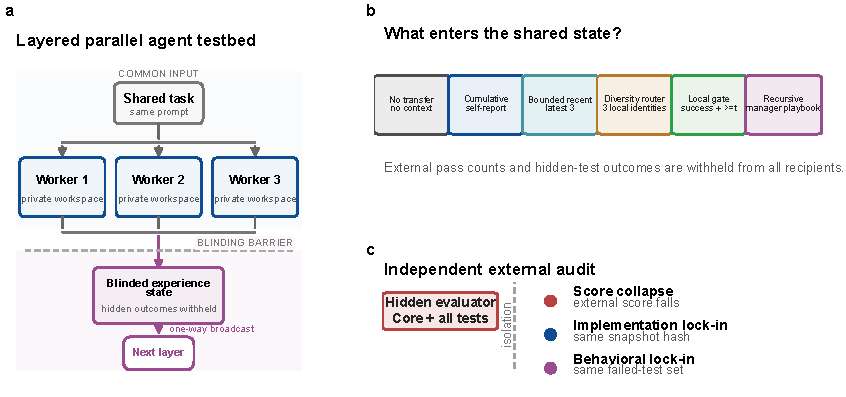
\includegraphics[width=\textwidth]{figures/moa/figure1_moa_system.pdf}
\caption{\textbf{可审计的分层并行智能体测试平台。}
\textbf{a}，三个 MiniSWE 工作者在私有工作区中并发解决同一任务；层间屏障关闭后，盲化经验状态才会广播到下一层。\textbf{b}，不同策略只改变进入共享状态的内容：不迁移、累积自报告、固定最近窗口、本地实现多样性路由、本地命令阈值接纳，或递归合成的管理器 playbook。\textbf{c}，隐藏评估器分别测量外部分数、实现身份和失败测试行为；外部结果不会提供给自报告或本地接纳的接收者。}
\label{fig:system-zh}
\end{figure*}

实现使用 AutoGen Core 的路由智能体运行时完成屏障与消息拓扑，并使用固定版本 SlopCodeBench 的原生 MiniSWE 运行器进行智能体--环境交互。参考答案、后续 checkpoint 规格及隐藏评估路径均从工作者可见空间中移除。每个被解释的结果都必须匹配冻结测试数和集合哈希，包含有效模型调用，并通过禁止访问扫描。

\subsection{迁移策略}

表~\ref{tab:policies-zh}定义各策略。\textbf{无迁移}屏蔽全部历史输出。\textbf{累积自报告}接纳轨迹中声称成功的所有输出，并把有长度上限的经验摘要追加到共享历史。\textbf{固定最近迁移}采用相同接纳信号，但始终只保留最近三条被接纳输出。\textbf{固定多样迁移}在启动源和已完成层中保留最近三个本地实现身份不同的输出。\textbf{本地接纳}额外要求至少三条成功环境命令；这是智能体本地的完成加冒烟代理，而不是外部验证。\textbf{递归合成}把当前被接纳输出与上一版共享 playbook 交给管理器，生成下一层唯一的修订 playbook。

\begin{table}[t]
\centering
\caption{迁移与接纳策略。“隐藏”表示外部评估结果不提供给接收者。}
\label{tab:policies-zh}
\begin{tabular}{p{0.20\columnwidth}p{0.32\columnwidth}p{0.25\columnwidth}}
\toprule
策略 & 共享状态 & 接纳信号 \\
\midrule
无迁移 & 空 & 无 \\
自报告 & 历史上全部已接纳摘要 & 声称成功 \\
固定最近 & 最近三条已接纳摘要 & 声称成功 \\
固定多样 & 最近三个本地不同实现 & 声称成功；本地源码哈希 \\
本地接纳 & 历史上全部已接纳摘要 & 声称成功且成功命令数 $\geq3$ \\
递归管理器 & 一个修订 playbook & 依探针采用自报告或外部 Core 门控 \\
\bottomrule
\end{tabular}
\end{table}

\subsection{经验制品与本地信号}

每个工作者生成一个有界文本制品，包含三个字段：工作者与层级头、最后四个 assistant 步骤末尾 6,000 个字符，以及 UTF-8 源码快照摘录；完整制品最终截断到 12,000 字符。接收提示将迁移制品标为可能出错的证据，并对每个来源独立应用同样上限。冻结主实验的累积臂中，制品中位长度为 10,479 字符；每个工作者收到的经验中位长度从第 1 层的 25,934 字符增长到第 12 层的 367,725 字符。

自报告接纳在全部 assistant 消息拼接文本上，以不区分大小写的单词边界匹配 \texttt{pass}、\texttt{passes}、\texttt{passed}、\texttt{works}、\texttt{working}、\texttt{success}、\texttt{successful}、\texttt{correct}、\texttt{verify} 和 \texttt{verified}。本地门控再要求至少三条成功环境命令。两者都不读取外部评估器。多样性路由器对本地实现文件做哈希，同时排除测试文件、缓存和评估器输出；它不增加模型调用，也不使用隐藏分数。精确正则表达式见补充材料。

\subsection{冻结主实验}

主实验通过同一 MaaS 提供商调用 Kimi-K2.6，在 \texttt{cfgpipe} checkpoint 1 上运行。该任务有 37 个可执行测试，其中 4 个构成 Core 子集。每臂包含三个工作者、12 层、每个工作者 12 步上限、温度 0.6，每个经验源最多 12,000 字符。两个迁移臂从同样的三个冻结多样化经验开始；每个经验都被独立复评为 Core 4/4、总体 34/37，但外部分数不会写入接收者提示。无迁移按定义不接收这些经验。

在新实验结果产生前，协议冻结三个主要问题：（i）累积自报告是否会产生至少两个后期 0/37 事件；（ii）无迁移是否产生更少此类事件；（iii）本地接纳是否拒绝所有零命令 0/37 输出，并阻止它们直接进入后续提示。全部 108 个工作者评估均通过目标一致性、模型调用完整性、提示盲化与禁止访问门控。

\subsection{前瞻对照与独立审计}

除冻结主实验外，我们把同一快照与失败测试审计回顾性地应用于两条独立累积自报告轨迹：一条 10 层 Kimi Coding 运行和一条 12 层 Kimi MaaS 运行。由于锁定指标并未为这些历史轨迹预注册，它们是复现审计，而不是独立的推断样本。更早的一条 Coding 轨迹曾向启动经验暴露 Core 分数，仅保留为协议漂移诊断，不计入复现。

我们还在观察结果前冻结一条新的六层 MaaS 对照。它匹配主实验的自报告语义，但每层只广播最近三条被接纳摘要。预先规定的判据是：截至第 6 层，至少连续两层的三个有效快照字节完全相同。该对照检验累积引用数量增长是否必要，但不把全部输入 token 与无迁移严格配平。

在审计该对照后，我们又在新结果产生前冻结一个只使用本地信号的多样性路由器。\texttt{cfgpipe} 协议复用已经冻结的无迁移与固定最近对照，只运行新的六层策略臂；协议明确披露控制复用以及控制结果已知。主要终点是第 2--6 层主实现多样性 AUC。随后，我们冻结一个紧凑的同提供商 \texttt{log\_query} 三臂边界：三层、两个迁移臂使用相同启动源，并且不依据中间结果提前停止。

\subsection{机制探针与边界}

我们在 \texttt{cfgpipe} 上分析两个递归管理器压力探针。Kimi 探针仅允许 Core 4/4 输出进入管理器，并配有匹配的无迁移臂。DeepSeek-V4-Flash 探针按自报告接纳，并有意使用一个完整且对分数盲化的启动 cohort；其仅用于审计的外部结果为 0/37、33/37 和 34/37。后者测试混合质量经验的压缩，不能证明全局正确经验本身会被放大成错误。

边界实验把递归合成应用于 \texttt{log\_query}、\texttt{xjq}，以及顺序 \texttt{cfgpipe} 或 \texttt{execution\_server} checkpoint。若控制臂被动作边界截断，则结果只作描述，不用于确认性效应声明。另一个 \texttt{log\_query} 边界比较严格 Core 门控的累积迁移与无迁移，并审计终端快照多样性。

\subsection{指标与决策纪律}

工作者 $i$ 在第 $\ell$ 层的外部分数定义为 $s_{i\ell}=p_{i\ell}/m$，其中 $p$ 为通过测试数，$m$ 为冻结测试总数。我们报告层均值和工作者范围；灾难事件严格定义为 0/$m$。

实现多样性分两级报告：全工作区哈希覆盖所有提交文件；主实现哈希只覆盖任务入口文件（\texttt{cfgpipe.py} 或 \texttt{logql.py}），避免把无关草稿或测试文件误判为新实现。新的前瞻路由和任务边界使用主实现哈希；历史复现保留原有全工作区审计。行为多样性由失败测试集合 $F_{i\ell}$ 表示，并报告唯一签名数、主导签名占比与平均两两 Jaccard：
\[
J_\ell=\frac{1}{3}\sum_{i<j}
\frac{|F_{i\ell}\cap F_{j\ell}|}{|F_{i\ell}\cup F_{j\ell}|}.
\]
协调负载由接收引用数、经验字符数和相对无迁移的输入 token 倍率衡量。

机制审计还把每个接收者实现与其收到的全部先前来源比较，测量主文件精确匹配、归一化源码行 Jaccard、函数名重叠、AST 节点数签名、字符串字面量，以及接收者源码行能否在已交付快照摘录中逐字找到。这些是对齐测量，而不是复制行为的因果估计。

每次运行都是一条耦合轨迹，每层三个工作者受到共享历史影响，层不是独立随机种子。因此本文报告精确描述统计，不进行把层伪装成独立样本的显著性检验。两条历史锁定复现是回顾性审计；跨模型或跨提供商运行分开呈现，不合并成可交换试验。

\begin{figure*}[t]
\centering
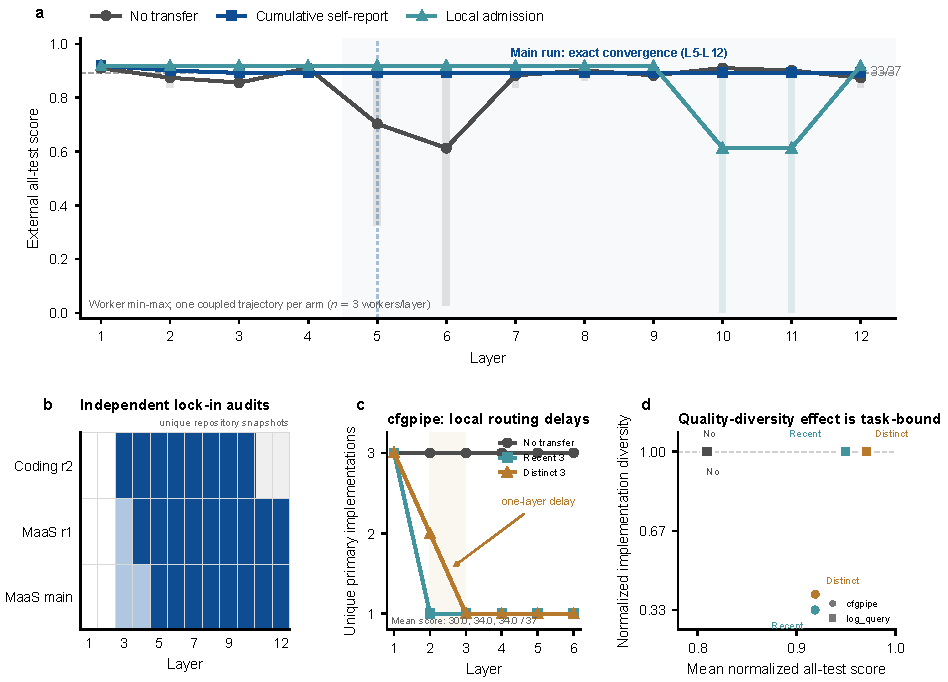
\includegraphics[width=0.90\textwidth]{figures/moa/figure2_depth12_lockin.pdf}
\caption{\textbf{实现吸引子可复现、只能被轻微缓解，并具有任务边界。}
\textbf{a}，冻结主实验的外部全测试分数；范围表示三个工作者的最小值与最大值。\textbf{b}，两条回顾性累积复现和冻结主实验中的唯一全工作区快照数；深色单元表示三个工作者精确收敛。\textbf{c}，前瞻 \texttt{cfgpipe} 主实现多样性。固定最近路由从第 2 层锁定；本地多样性路由在第 2 层保留两个实现，但从第 3 层锁定，且质量不变。\textbf{d}，平均标准化分数与第 1 层后标准化主实现多样性。迁移在两个任务上都提高分数，但只在 \texttt{cfgpipe} 上降低多样性；圆点表示 \texttt{cfgpipe}，方块表示前瞻冻结、同提供商的 \texttt{log\_query} 边界。所有面板都是耦合轨迹的描述结果，而非独立随机种子。}
\label{fig:main-zh}
\end{figure*}

\section{结果}

\subsection{RQ1：持续退化没有被复现}

图~\ref{fig:main-zh}a 展示冻结的 12 层结果。累积自报告从第 1 层 34/37 降到第 3 层三个工作者均值 33/37，随后一直保持到第 12 层，并且没有产生任何 0/37 事件。因此，预注册的反复灾难尾部复现被否定。

两个控制也不支持“迁移独有灾难”。无迁移在第 5、6 层出现有效的动作预算尾部，分别为 12/37 和 1/37，之后恢复。本地接纳在第 10 层和第 11 层各出现一个 0/37 工作者，使两层均值降到 0.613，但第 12 层所有工作者又回到 34/37。两个本地臂事件都是独立的假完成轨迹而非传播快照：每个只有一次模型步骤，执行零条命令，不生成快照，并被门控拒绝。

在累积自报告的跨模型运行中，DeepSeek-V4-Flash 有 2/30 个零分事件，GLM-5 为 0/30，Kimi-K2.6 在初始 coding endpoint 运行中为 1/24，而在预注册复现和新 MaaS 复现中分别为 0/30 与 0/36（图~\ref{fig:boundaries-zh}b）。所有有效零分事件要么孤立、要么发生在终点，没有一例建立持续下降曲线。增加层数只会提高抽样到稀有失败的机会，不能单独解释持续退化。

\subsection{RQ2：共享经验消除了独立解}

没有死亡螺旋并不意味着迁移没有作用。图~\ref{fig:main-zh}b--c 显示快速收敛。在累积自报告中，从第 3 层到第 12 层，三个工作者始终共享同一个失败测试签名。第 3--4 层仍有两个快照哈希；从第 5 层起，剩余 24 个输出的目录快照完全相同。第 3--12 层每个工作者都通过 Core，并失败于同样的四个更广测试。

第 12 层时，无迁移仍保留三个不同快照、三个失败测试签名，主导快照占比为 $1/3$，失败测试两两 Jaccard 为 0.278。累积自报告与本地接纳都以一个快照、一个签名、主导占比 1 和 Jaccard 1 结束。因此，本地接纳会拦截部分轨迹，却不能保护被接纳轨迹之间的终端实现多样性。

相同的实现现象也出现在主轨迹之外（图~\ref{fig:main-zh}c）。独立 Coding 运行在第 2 层仍有三个快照，第 3--10 层则只剩一个共享快照。独立 MaaS 运行在第 4--9 层收敛为一个快照，第 10 层出现一次无快照的 0/37 事件，并在第 11 层重新收敛。两个匹配的无迁移控制均未出现连续两层精确收敛。

前瞻固定最近臂把锁定与累积历史增长分开（图~\ref{fig:main-zh}c）。第 1 层包含三个不同的 34/37 主实现；第 2--6 层，每个工作者只接收三条引用，却都生成完全相同的 \texttt{cfgpipe.py}。第 4 层和第 6 层的全工作区哈希差异只来自辅助 \texttt{ws.txt} 或测试文件，并不代表主实现重新分化。在首次锁定的两层，其总输入仅为匹配无迁移的 1.26--1.60 倍，而累积臂第 12 层达到 14.08 倍。因此，累积数十条引用并非锁定的必要条件，但迁移上下文本身仍是合理贡献因素。

交付制品包含异常直接的实现证据。第 1 层之后，87.9\% 的累积臂接收者与至少一个先前主实现精确相同；它们与来源的最大源码行 Jaccard 均值为 0.965，并且 97.6\% 的接收者源码行可以在至少一个已交付快照摘录中逐字找到。固定最近臂的三项指标均为 1.0。这些结果支持实现吸引子机制，但不能区分逐字复制与在相同富代码提示条件下的确定性再生成。

\subsection{RQ3：本地多样性路由只能推迟锁定}

前瞻本地路由器仍保持三引用上限，但会在所有启动源和历史层中选择最近三个实现身份不同的输出。在 \texttt{cfgpipe} 上，固定最近臂第 2--6 层的多样性 AUC 为理论最小值 5，精确主实现锁定从第 2 层开始。多样性路由把 AUC 提高到 6：第 2 层保留两个实现，但第 3--6 层仍锁定。两个迁移臂的全部 18 个输出均为 34/37，因此这只是没有质量代价的一层延迟，而不是解决方案。

前瞻冻结、同提供商的 \texttt{log\_query} 探针是任务边界，而不是锁定复现（图~\ref{fig:main-zh}d）。无迁移、固定最近和固定多样三臂在每个测量层都保留三个主实现；平均全测试通过数分别为 108.4/134、127.2/134 和 130.1/134，两个迁移臂的平均 Core 均为 9.67/10。由于固定最近已经达到多样性上限，无法识别多样性路由的增量缓解效应。\texttt{cfgpipe} 吸引子因此依赖任务与具体轨迹，而不是共享经验的自动后果。

\begin{figure*}[t]
\centering
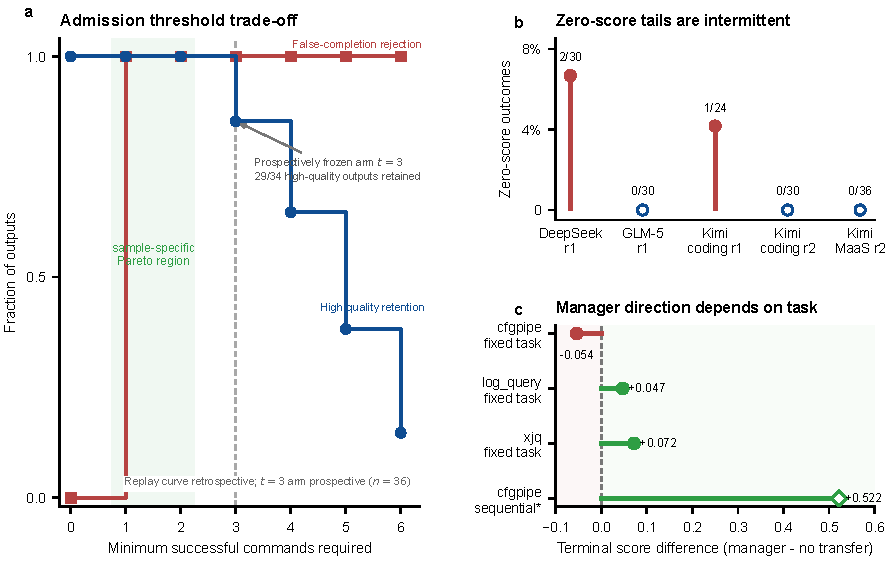
\includegraphics[width=\textwidth]{figures/moa/figure3_admission_boundaries.pdf}
\caption{\textbf{接纳质量与结果方向具有条件性。}
\textbf{a}，对本地臂全部 36 个输出进行回顾性阈值回放：灾难拒绝率是两个 0/37 输出中被拒绝的比例，高质量保留率是 34 个至少 33/37 输出中被接纳的比例。回放曲线是回顾性的，但标出的三命令实验臂在结果产生前已经冻结；阴影阈值只对本样本成立，不是经验证的普适最优值。\textbf{b}，五次累积自报告模型运行中的有效零分事件（共 150 个工作者输出）；由于层和提供商不可交换，事件率分开报告。\textbf{c}，递归管理器设置下终端“处理减无迁移”分数差。顺序 \texttt{cfgpipe} 控制有噪声并以星号标记；这些效应不进行合并。}
\label{fig:boundaries-zh}
\end{figure*}

\subsection{RQ4：递归合成可以赋予固定点特权}

递归管理器探针说明，紧凑且有特权的共享制品如何稳定共同错误。在 Kimi \texttt{cfgpipe} 探针中，管理器第 3 与第 4 层 playbook 字节完全相同。第 5 层所有递归工作者生成同一快照并得到 32/37；无迁移的三个工作者则生成三个不同快照并得到 34/37。管理器持续保留一个错误的来源优先级规则及另外两个边界错误。这支持固定点锁定机制，但预注册的 Core 主效应被否定，因为两臂都保持 4/4 Core。

DeepSeek 压力探针形成近似文本固定点。三个终端实现彼此不同，却都得到 32/37 并失败于同样五个测试。由于启动 cohort 包含一个外部失败源，该结果只能证明合成会把混合质量轨迹压缩成共同行为，不能证明局部或全局正确经验本身必然有害。

方向并不跨任务一致（图~\ref{fig:boundaries-zh}c）。递归合成在 \texttt{log\_query} 上将终端标准化全测试分数提高 0.047，在 \texttt{xjq} 上提高 0.072。顺序 \texttt{cfgpipe} 试验相对一个受动作预算影响的噪声控制提高 0.522。\texttt{execution\_server} 试验在描述上为正，但无迁移在冻结动作边界处没有明确提交，因此确认性无效。共享固定点既可能编码有用稳定性，也可能编码共同错误；方向取决于任务和接纳语义。

\subsection{RQ5：接纳会拦截假完成，也会付出代价}

本地门控的三命令阈值在 36 输出实验臂运行前已经冻结。它拒绝两个观察到的 0/37 假完成，并且其制品标识从未出现在后续接收提示中。这是在所审计实验臂中对直接传播的前瞻机械保护。

同一门控在 36 个输出中拒绝 7 个：两个 0/37，以及五个只使用两条成功命令、但外部达到 34/37 的强解。我们在冻结轨迹上回放阈值 0--6（图~\ref{fig:boundaries-zh}a）。在本样本中，阈值 1 或 2 能保留全部 34 个高质量输出，同时拒绝两个零命令事件；冻结阈值 3 只保留 29/34 个高质量输出。这是回顾性敏感性结果，不说明“两条命令”是普适最优值。它说明接纳质量依赖阈值校准，“更多验证”并非无成本。

\section{讨论}

\paragraph{主要风险是可选性的丧失。}
并行智能体的价值部分来自不同轨迹探索不同实现和失败模式。在主实验中，迁移在造成灾难分数下降之前就消除了这种可选性。只报告平均成功率的系统可能看起来健康，却让所有工作者共享同一个盲点。实现多样性和失败测试多样性应成为多智能体编程系统的伴随指标。

\paragraph{稳定性和多样性都不是单调的善。}
同提供商任务边界说明，不能把同质化一般化为必然或有害。在 \texttt{log\_query} 上，共享经验提高分数，却没有降低实现多样性。工程目标不是最大化多样性，而是\emph{经验证的多元性}：在证据足够支持收敛之前，保留真正不同的候选方案。

\paragraph{去重本身不是充分的缓解。}
本地多样性路由只改变一个机制变量，不使用隐藏评估，也不增加模型调用，但在 \texttt{cfgpipe} 上只争取到一层。一旦所有接收者看到相同的富代码经验包，不同来源仍可能诱导同一首选实现。更强的缓解可能需要接收者异质性、反事实任务划分、主动寻求分歧的提示，或显式组合优化目标，而不仅是路由去重。

\paragraph{接纳是治理问题。}
自报告会接纳明显假完成；命令数门控能捕获观察到的零命令案例，却会把“工作简洁”与“根本没工作”混为一谈。更好的接纳机制应结合来源、任务相关本地测试、代码变更证据、不确定性和对多样性的贡献，并保留被拒制品以供审计，而不是静默删除。

\paragraph{更多层不一定是更好的机制检验。}
一旦共享 playbook 或快照到达固定点，继续运行同样的层主要是在重新抽样随机执行并膨胀上下文。更强的因果检验应在匹配控制下改变一个机制变量，例如接纳、压缩、路由或接收者异质性，而不是延长已经平稳的曲线。

\section{局限性}

最强的确认性结果仍来自一个 Kimi 提供商、一个 \texttt{cfgpipe} checkpoint 和每层三个工作者的一次冻结运行。两条独立累积轨迹回顾性地复现精确锁定，但该指标没有预注册，也不构成推断抽样分布。固定上下文对照只有一条前瞻轨迹，且没有严格配平所有输入 token。多样性路由臂复用已经观察过的冻结控制，只有一条轨迹，并且只检验精确本地身份去重。同提供商 \texttt{log\_query} 边界虽然是前瞻的，但仅运行三层，因此不能排除更深层的后续锁定。两个前瞻探针都没有独立随机种子、更大工作者群体、温度扫描或异构模型。跨模型审计使用不同提供商端点，并非同一不可变模型二进制的统计复现。SlopCodeBench 任务可执行且足以暴露编程行为，但不覆盖浏览器办公、长期组织或异步智能体。递归探针的接纳语义不同；DeepSeek 探针包含混合质量启动源，部分顺序控制受到动作预算噪声或截断。门控实验臂是前瞻的，但阈值扫描是回顾性的。全工作区哈希会因无关辅助文件而高估实现差异，因此新的前瞻终点采用主入口文件哈希，但历史复现仍保留完整快照口径。失败测试一致也可能漏掉评估器未覆盖的潜在差异。因此，本文只主张一个有边界、可审计的失效模式和权衡，而不是多智能体学习的普适定律。

\section{结论}

反复共享经验没有产生我们原先寻找的、行军蚁式持续退化曲线。实验得到的是一个更可辩护的结论：并行编程智能体可以迅速失去实现和行为独立性，反复进入共享实现吸引子，同时仍维持看似较强的总体分数。精确锁定在三条累积轨迹中重复出现，也出现在固定三引用对照中，因此在所测设置里，累积历史增长不是必要条件。本地身份感知路由只把锁定推迟一层，没有阻止它。前瞻冻结、同提供商的 \texttt{log\_query} 边界在迁移提高质量时仍保留最大的实现多样性，表明该吸引子依赖任务而非普适存在。灾难尾部事件是间歇且依赖模型的；递归合成可能有益也可能有害；本地接纳只有在选择一个带误拒成本的阈值后才能阻断假完成。因此，多智能体系统不应只评估共享经验是否提高平均分，还应评估它消除了什么多样性、由什么证据接纳，以及缓解措施能否持续超过下一层。

\bibliographystyle{aaai2027}
\bibliography{antmill}

\end{document}
